\chapter{Návrh}

V této kapitole se budu věnovat návrhu knihovny na automatizaci a jejím funkčním požadavkům.

\section{Zařízení}
V rámci knihovny a testovacího běhu se bude vyskytovat několik účastníků. Tyto participanti budou:

\begin{description}
    \item[Testovací zařízení] Hlavní zařízení, ze kterého poběží testovací služba.
    \item[Fyzický participant] Fyzické zařízení, které běží mimo zařízení s testovací službou. 
    \item[Virtuální participant] Zařízení, které simuluje protistranu fyzickým participantům. Toto zařízení běží na stejném zařízení jako testovací služba.
\end{description}

Hlavním cílem je testovat vyvíjený produkt. V kontextu této knihovny ho budeme nazývat fyzický participant. Do této kategorie avšak také bude patřit jakékoliv zařízení, které běží mimo zařízení, které řídí testování. Tato zařízení budou k zařízení, které řídí testovaní, připojena za pomoci Ethernet připojení.

Knihovna zároveň bude obsahovat tzv. virtuálního participanta. Toto zařízení bude sloužit k simulaci protistrany u testování fyzického zařízení. Je to volitelný participant. Zároveň může být během testu připojeno více virtuálních participantů. Simulováním participanta snižujeme hardwarové nároky na testování, což vede ke snížení ekonomických nákladů na testování. Tito participanti se budou připojovat před započnutím určitého testu a po skončení tohoto jednoho testu zaniknou.

Testovací služba poběží na samostatném zařízení. Toto zařízení bude běžet na operačním systému Windows. Toto zařízení bude v rámci infrastruktury serveru Azure DevOps tzv. agent. Agent je výpočetní infrastruktura s nainstalovaným softwarem agenta, který pracuje na jedné určité úloze \cite{agent_docs}. Na agentovi bude server Azure DevOps spouštět testovací běh.

Testovací knihovna a virtuální participant budou vyvinuti v jazyce \inlinecode{C\#}. Jazyk byl vybrán kvůli dobrému rozsahu již implementovaných komponent a kvůli dobré interoperabilitě se serverem Azure DevOps, díky tomu že obě části jsou vyvíjeny společností Microsoft. Rozhraní pro vyvíjený produkt bude vytvořeno v jazyce \inlinecode{C++}, jelikož tento produkt je v tomto jazyce vyvíjen.


\section{Komunikace}
Komunikace mezi participanty bude fungovat na principu TCP/IP připojení. Zároveň zprávy, které budou mezi službou a participanty vyměňovány, budou mít stanovenou strukturu. Jedna zpráva bude obsahovat délku zprávy, typ zprávy a poté data zprávy. Data zprávy se budou odvíjet od typu zprávy. Existují i situace, kdy zpráva žádná data obsahovat nebude, k přenesení informace tedy bude stačit pouze typ zprávy. 

Složení zprávy lze vidět na obrázku \ref{fig:message}. Všechny hodnoty budou ukládány v kladné (anglicky tzv. unsigned) podobě. Z diagramu lze vidět, že jedna zpráva bude mít maximální délku rovna číslu, které se vejde do dvou bajtů, tedy maximální délka jedné zprávy je 65~535 bajtů. Tato délka je ale více než dostatečná pro navrhované použití.  

\begin{figure}[htbp]
    \centering 
    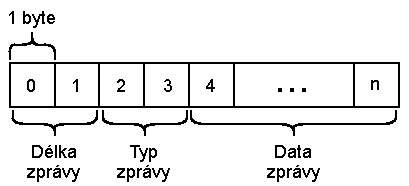
\includegraphics{assets/img/message.pdf}
    \caption{Diagram struktury jedné zprávy}
    \label{fig:message}
\end{figure}


\section{Služba}
Ve vyvíjené knihovně bude jádrem k řízení testování služba, která se bude starat o běh testování. Služba v počáteční fázi vytvoří připojení se všemi fyzickými participanty testu. Po připojení určitého počtu očekávaných participantů započne samotné testování. Služba bude spouštět testy a během testu bude synchronizovat stádia testování mezi všemi participanty testu. Následně po běhu testu vyhodnotí úspěšnost testu na základě dat, které obdrží od participantů. 


\section{Rozhraní pro testování}
Součástí knihovny taktéž bude rozhraní, pro implementaci zařízení, které bude testováno. Toto rozhraní bude mít jasně definovanou  strukturu, ale zároveň bude co nejjednodušší pro co nejrychlejší implementaci na nově testovaném zařízení. Toto rozhraní bude potom využito pro řízení běhu testu na testovaném zařízení. 

Další součástí bude i rozhraní pro jednotlivé testy. To bude obsahovat jednotlivá stádia testování, která budou mezi všemi zařízeními synchronizovány. Tyto stádia budou, v tom pořadí:
\begin{enumerate}
    \item Příprava na testování
    \item Samotné testování
    \item Úklid po testu
\end{enumerate}

\section{Proces testování}

Ze předchozí definice testování vyplývá, že knihovna je mířena na automatizaci funkčního testování. Každý testovací běh se bude moc skládat z libovolného počtu registrovaných testů. Na obrázku \ref{fig:act_diag_device} můžeme vidět diagram aktivit testovaného zařízení. Samotné kontrolování správnosti testu bude prací jednotlivých testerů. Knihovna pouze dostane informaci o úspěchu nebo neúspěchu jednotlivých synchronizačních částí testovaní, definovaných rozhraním pro testování. Pokud ve fázi přípravy na testování nebo úklidu po testu zařízení vrátí neúspěch, bude toto zařízení považováno jako v chybném stavu. Další testy poté nebudou provedeny. 

\begin{figure}
    \centering 
    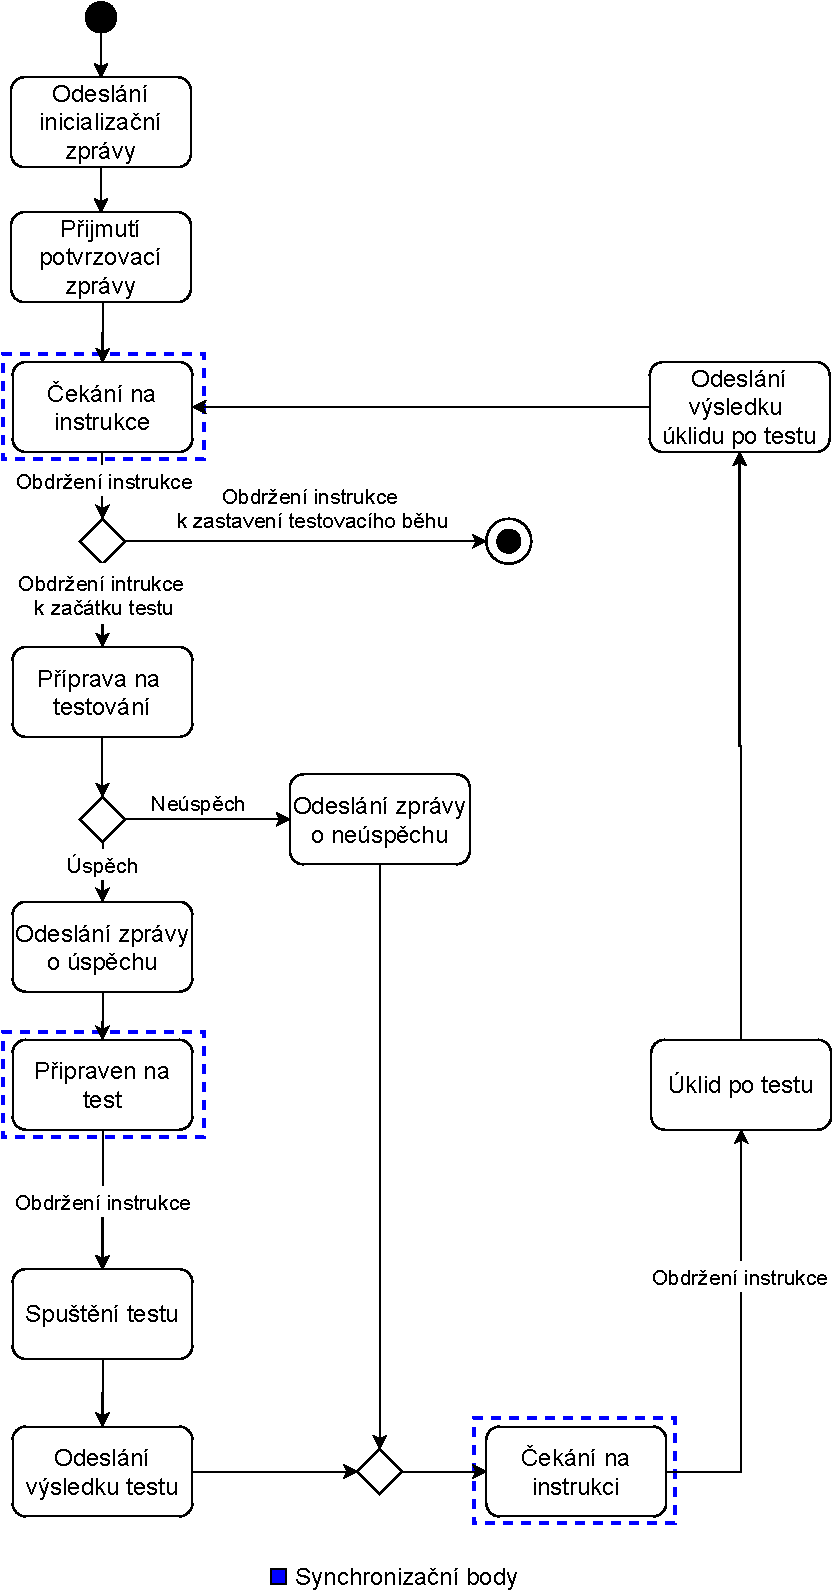
\includegraphics[width=\textwidth]{assets/img/activitydiagramdevice.pdf}
    \caption{Diagram aktivit testované zařízení}
    \label{fig:act_diag_device}
\end{figure}

\section{Propojení se serverem Azure DevOps}
Jedním z cílů této práce je vytvoření takového připojení, aby server Azure DevOps byl schopen spouštět jednotlivé testy. K tomuto propojení využijeme testovací framework MSTest. Vyvíjená testovací knihovna tedy poběží nad tímto testovacím frameworkem. Za pomoci frameworku MSTest bude server Azure DevOps schopen registrovat jednotlivé testy, a spouštět je jednotlivě.

